\documentclass[11pt]{article}

\input{../../Latex_Common/skinnerr_latex_preamble_asen5417.tex}

%%
%% DOCUMENT START
%%

\begin{document}

\pagestyle{fancyplain}
\lhead{}
\chead{}
\rhead{}
\lfoot{\hrule ASEN 5417: Homework 8}
\cfoot{\hrule \thepage}
\rfoot{\hrule Ryan Skinner}

\noindent
{\Large Homework 8}
\hfill
{\large Ryan Skinner}
\\[0.5ex]
{\large ASEN 5417: Numerical Methods}
\hfill
{\large Due 2015/12/8}\\
\hrule
\vspace{6pt}

%%%%%%%%%%%%%%%%%%%%%%%%%%%%%%%%%%%%%%%%%%%%%%%%%
%%%%%%%%%%%%%%%%%%%%%%%%%%%%%%%%%%%%%%%%%%%%%%%%%
\section{Introduction} %%%%%%%%%%%%%%%%%%%%%%%%%%
%%%%%%%%%%%%%%%%%%%%%%%%%%%%%%%%%%%%%%%%%%%%%%%%%
%%%%%%%%%%%%%%%%%%%%%%%%%%%%%%%%%%%%%%%%%%%%%%%%%

Consider the linear convection-diffusion equation
\begin{equation}
\pp{T}{t} + v \pp{T}{y} = \alpha \pp{^2T}{y^2}
\;, \qquad
v = \sin(\pi y)
\;, \qquad
\alpha = \frac{1}{\text{Pr}\;\text{Re}}
\;,
\label{eq:conv-diff}
\end{equation}
subject to the initial conditions
\begin{equation}
\begin{aligned}
\text{(a)} && T(y,t=0) &= \cos(2 \pi y) \sin(\pi y) \\
\text{(b)} && T(y,t=0) &= \cos(2 \pi y)
\;,
\end{aligned}
\end{equation}
and parameters
\begin{equation}
\begin{aligned}
\text{Re} &= 1 &\quad &\text{(Reynolds number, molten glass)} \\
\text{Pr} &= 25 &\quad &\text{(Prandtl number, molten glass)} \\
\Delta t &= 0.001 &\quad &\text{(Time step)} \\
L_y &= 2 &\quad &\text{(Domain $y$-length)} \\
N &= 2^n + 1 &\quad &\text{(Number of $y$-points, where $n=5,6$)}
\;.
\end{aligned}
\end{equation}

\subsection{Problem 1}

Use the Fourier pseudo-spectral method to numerically integrate \eqref{eq:conv-diff} with the given parameters. Use the Euler explicit method for time advancement. Higher resolution with $n=6$ will improve the accuracy of the method for the initial condition (a). Plot $T$ as a function of time $t$ at $t = \{0.2, 2, 5, 10\}$.

\subsection{Problem 2}

Use the FTCS Euler explicit method with second-order finite differences for the same computation, and compare results to the Fourier pseudo-spectral method using the same mesh resolution.

%%%%%%%%%%%%%%%%%%%%%%%%%%%%%%%%%%%%%%%%%%%%%%%%%
%%%%%%%%%%%%%%%%%%%%%%%%%%%%%%%%%%%%%%%%%%%%%%%%%
\section{Methodology} %%%%%%%%%%%%%%%%%%%%%%%%%%%
%%%%%%%%%%%%%%%%%%%%%%%%%%%%%%%%%%%%%%%%%%%%%%%%%
%%%%%%%%%%%%%%%%%%%%%%%%%%%%%%%%%%%%%%%%%%%%%%%%%

\subsection{Problem 1}

We re-write \eqref{eq:conv-diff} as
\begin{equation}
\pp{T}{t} = \alpha \pp{^2T}{y^2} - v \pp{T}{y}
\;.
\end{equation}
The first and second spatial derivatives of $T$ are calculated by taking the Fourier transform of $T$, multiplying the Fourier coefficients by $i k_n$ and $-k_n^2$, respectively, and then taking the inverse Fourier transform. With values of $\partial T / \partial t$ known at all grid points now, values of $T$ at the next time step are calculated using the explicit Euler method,
\begin{equation}
T^{n+1} = T^n + \Delta t \pp{T}{t}
\;.
\end{equation}

\subsection{Problem 2}

To implement the FTCS explicit method, we approximate \eqref{eq:conv-diff} using forward-differences in time and central-differences in space as
\begin{equation}
\frac{T_i^{n+1} - T_i^n}{\Delta t}
+ v \frac{T_{i+1}^n - T_{i-1}^n}{2 \Delta y}
=
\alpha \frac{T_{i+1}^n - 2 T_i^n + T_{i-1}^n}{\Delta y^2}
\;,
\end{equation}
which can be solved for $T_i^{n+1}$ as
\begin{equation}
T_i^{n+1}
=
T_i^n +
\Delta t
\left(
\alpha \frac{T_{i+1}^n - 2 T_i^n + T_{i-1}^n}{\Delta y^2}
- v \frac{T_{i+1}^n - T_{i-1}^n}{2 \Delta y}
\right)
\;.
\end{equation}
This constitutes an explicit equation for $T^{n+1}$, and thus we can step forward in time without the need to solve any matrix equations. We enforce periodic boundary conditions by wrapping $T_{i-1}$ to $T_{N}$ when $i=1$ and vice versa.

%%%%%%%%%%%%%%%%%%%%%%%%%%%%%%%%%%%%%%%%%%%%%%%%%
%%%%%%%%%%%%%%%%%%%%%%%%%%%%%%%%%%%%%%%%%%%%%%%%%
\section{Results} %%%%%%%%%%%%%%%%%%%%%%%%%%%%%%%
%%%%%%%%%%%%%%%%%%%%%%%%%%%%%%%%%%%%%%%%%%%%%%%%%
%%%%%%%%%%%%%%%%%%%%%%%%%%%%%%%%%%%%%%%%%%%%%%%%%

\begin{figure}[p!]
\begin{center}
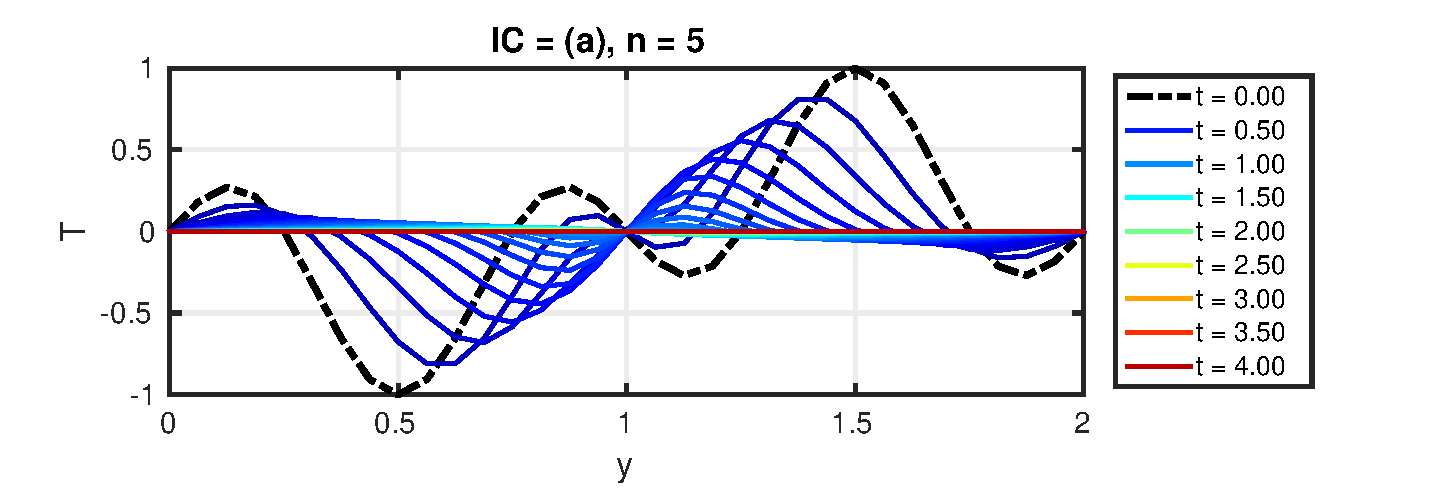
\includegraphics[width=0.85\textwidth]{Prob1_a5.eps} \\
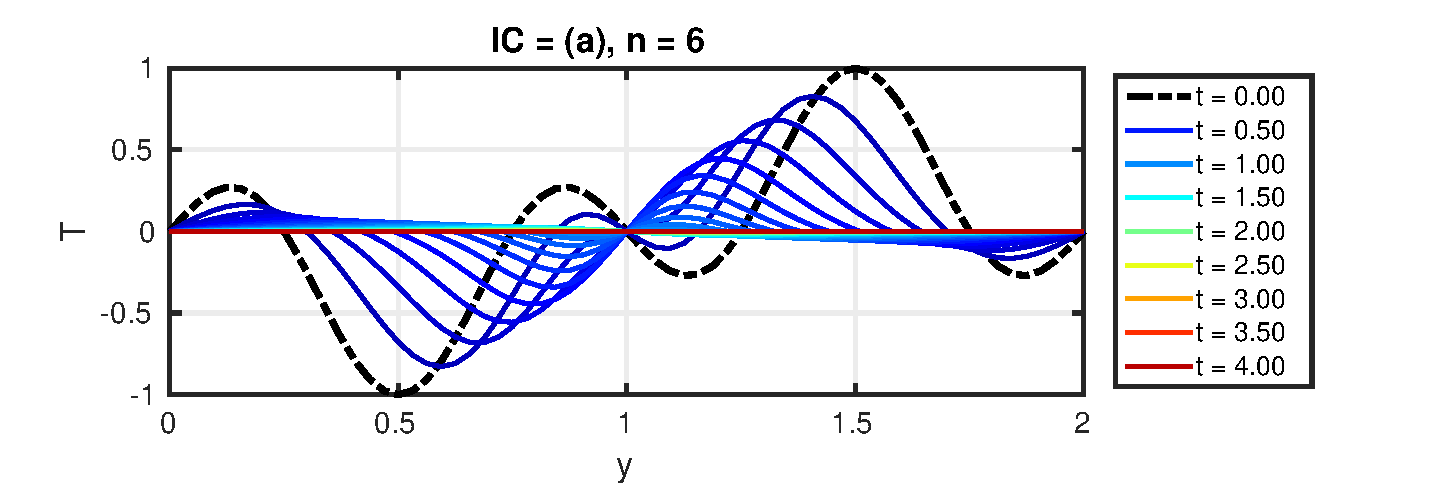
\includegraphics[width=0.85\textwidth]{Prob1_a6.eps} \\
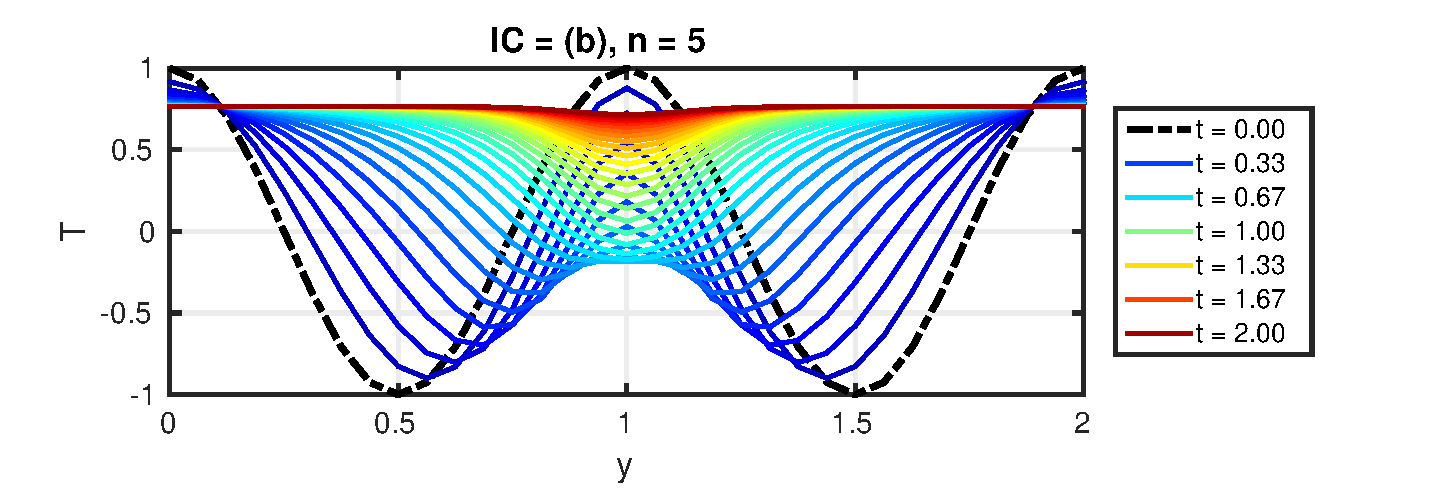
\includegraphics[width=0.85\textwidth]{Prob1_b5.eps} \\
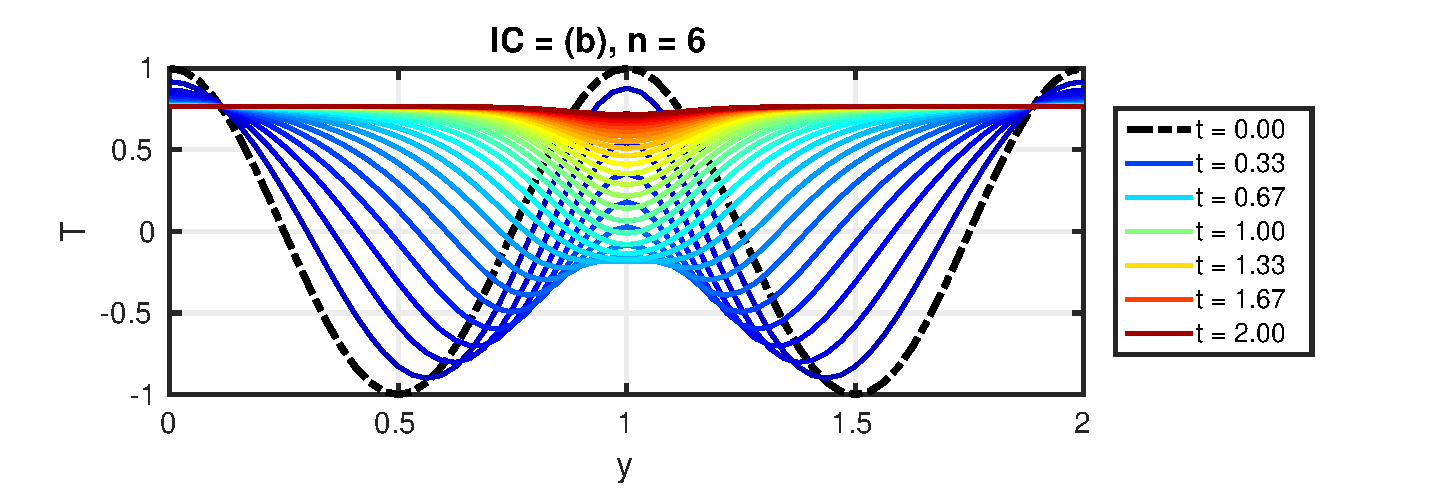
\includegraphics[width=0.85\textwidth]{Prob1_b6.eps}
\\[0.5cm]
\caption{Solutions to the linear convection-diffusion equation using the Fourier pseudo-spectral method for different initial conditions and mesh resolution parameters. Most interesting behavior occurs when $t<4$. Trends can be extrapolated to future times $t=5, 10$, which are not shown. Initial condition displayed as black dot-dashed line (\dotdashrule).}
\label{fig:Prob1}
\end{center}
\end{figure}

\begin{figure}[p!]
\begin{center}
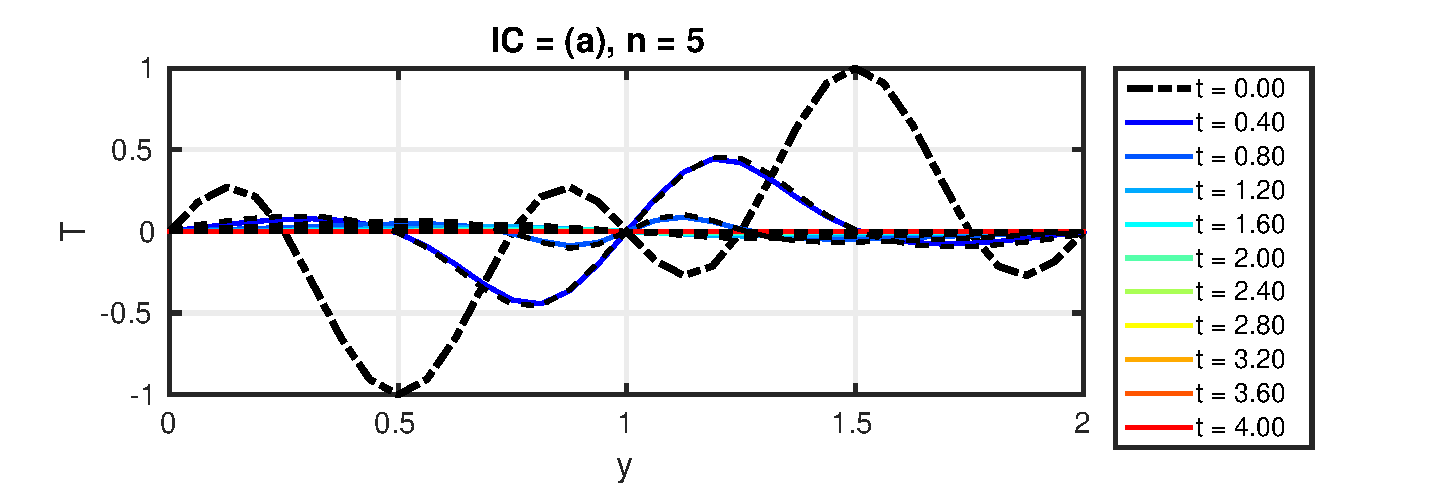
\includegraphics[width=0.85\textwidth]{Prob2_a5_comparison.eps} \\
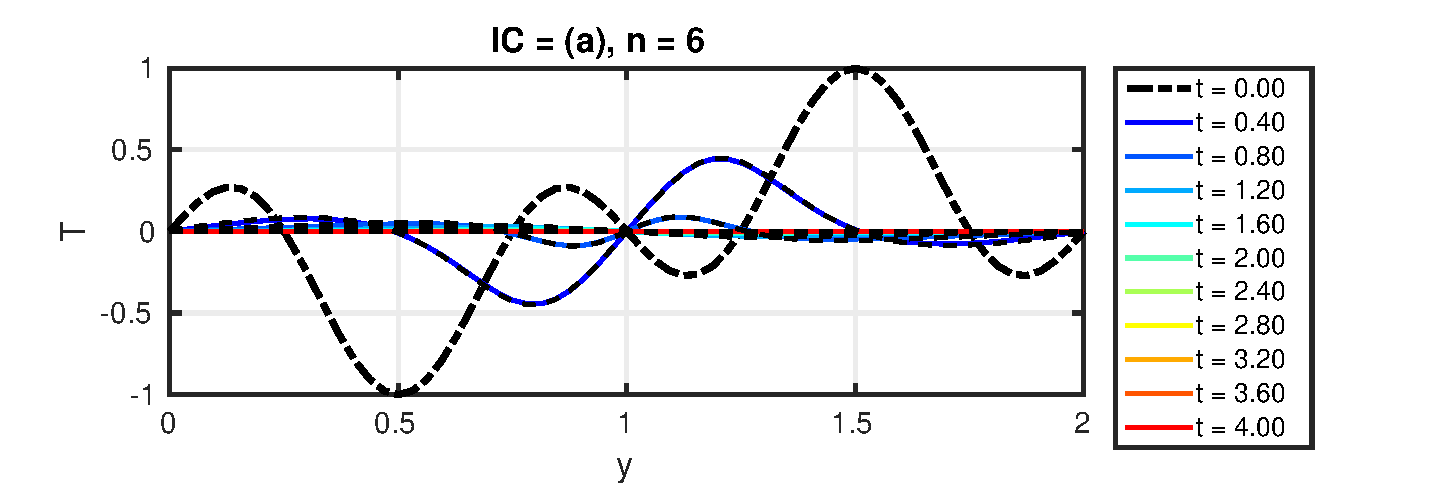
\includegraphics[width=0.85\textwidth]{Prob2_a6_comparison.eps} \\
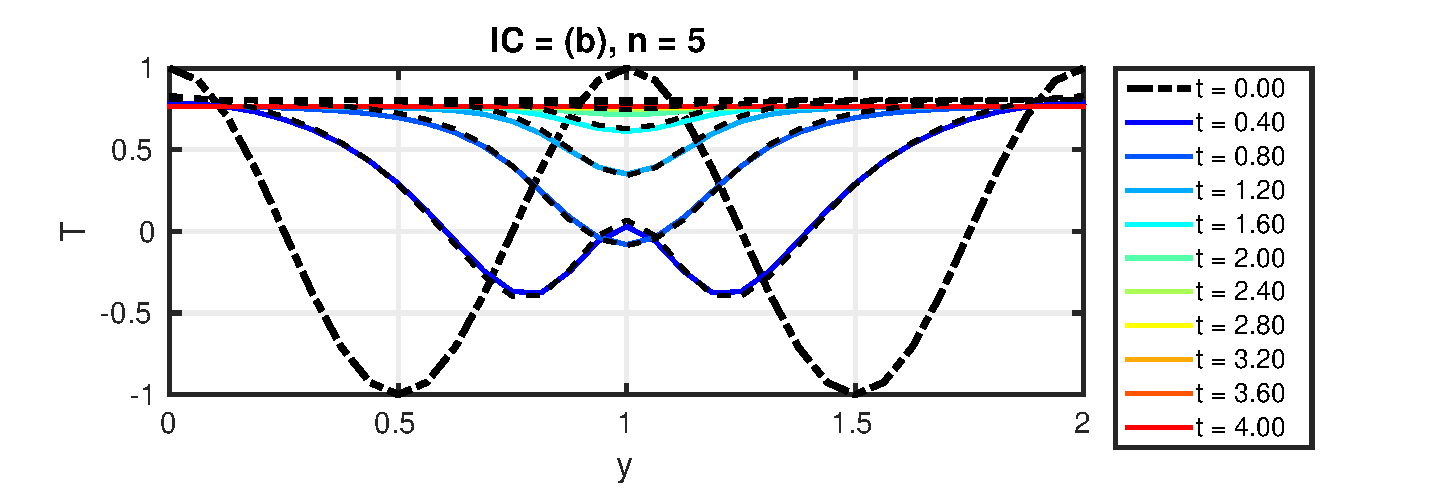
\includegraphics[width=0.85\textwidth]{Prob2_b5_comparison.eps} \\
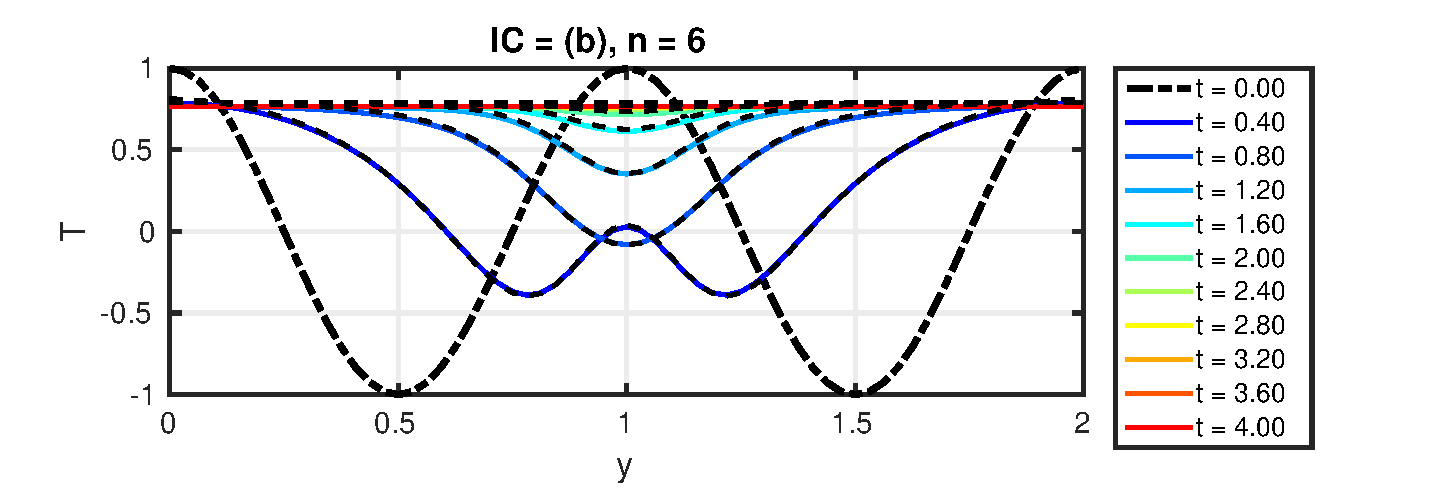
\includegraphics[width=0.85\textwidth]{Prob2_b6_comparison.eps}
\\[0.5cm]
\caption{Solution comparison between the Fourier pseudo-spectral method (colored lines) and the FTCS method (\dashrule) for $t<4$. Initial condition displayed as black dot-dashed line (\dotdashrule). Agreement between the Fourier and FTCS methods is decent. The limiting Fourier value is $T \sim 0.765$ for both $n=\{5,6\}$, whereas the FTCS method's limiting values are $T \sim \{0.806, 0.788\}$ respectively. Further analysis is deferred to \figref{fig:Prob2_error}.}
\label{fig:Prob2_comparison}
\end{center}
\end{figure}

\begin{figure}[p!]
\begin{center}
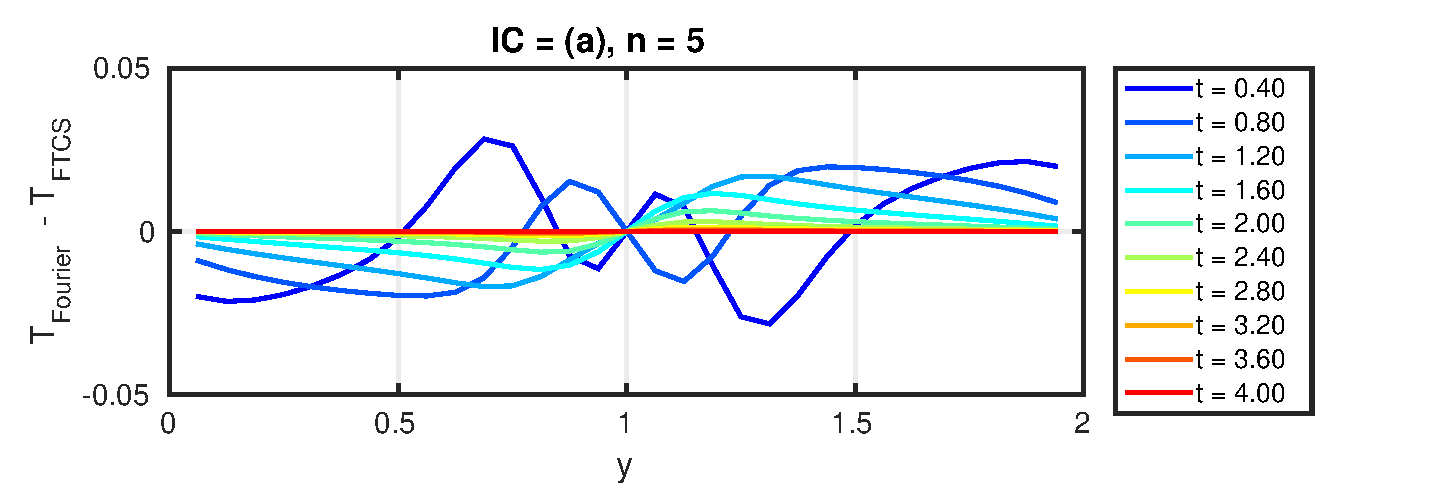
\includegraphics[width=0.85\textwidth]{Prob2_a5_error.eps} \\
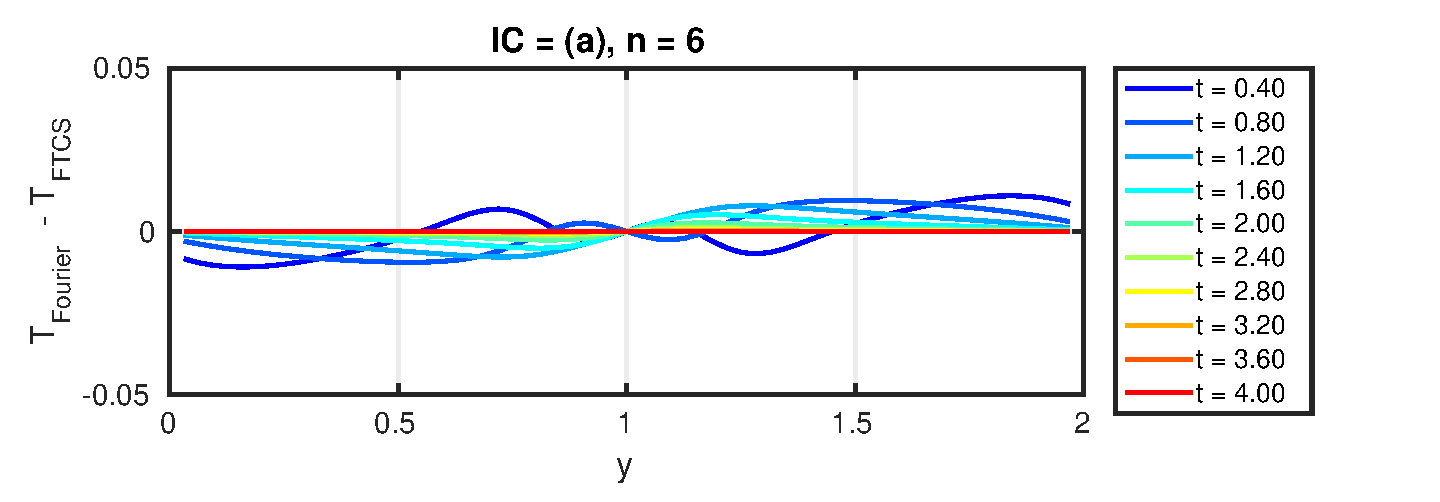
\includegraphics[width=0.85\textwidth]{Prob2_a6_error.eps} \\
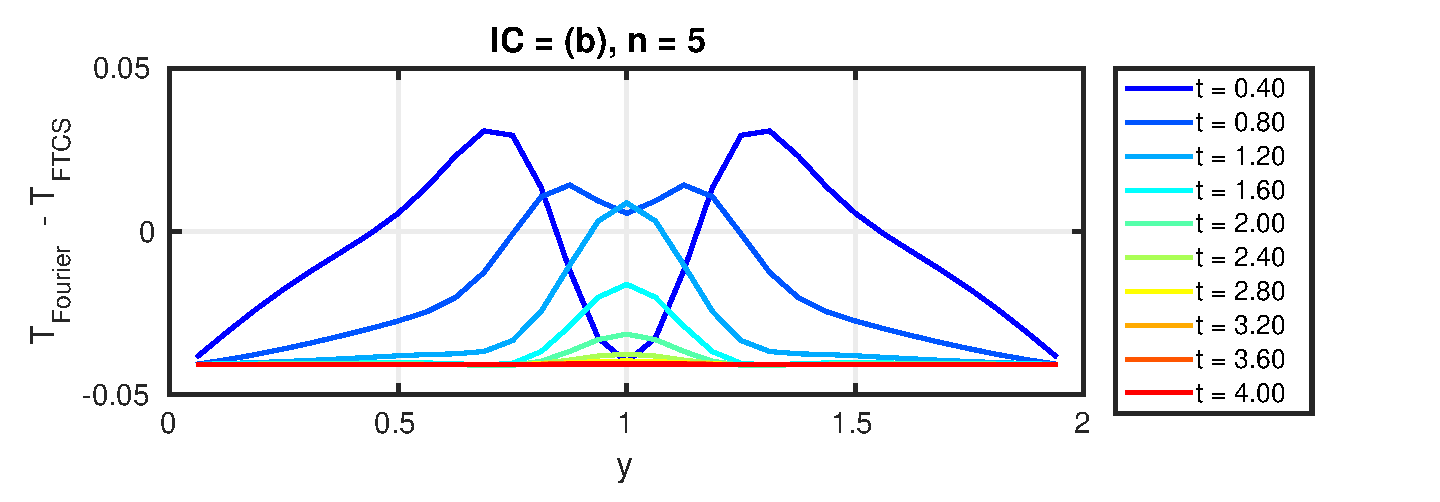
\includegraphics[width=0.85\textwidth]{Prob2_b5_error.eps} \\
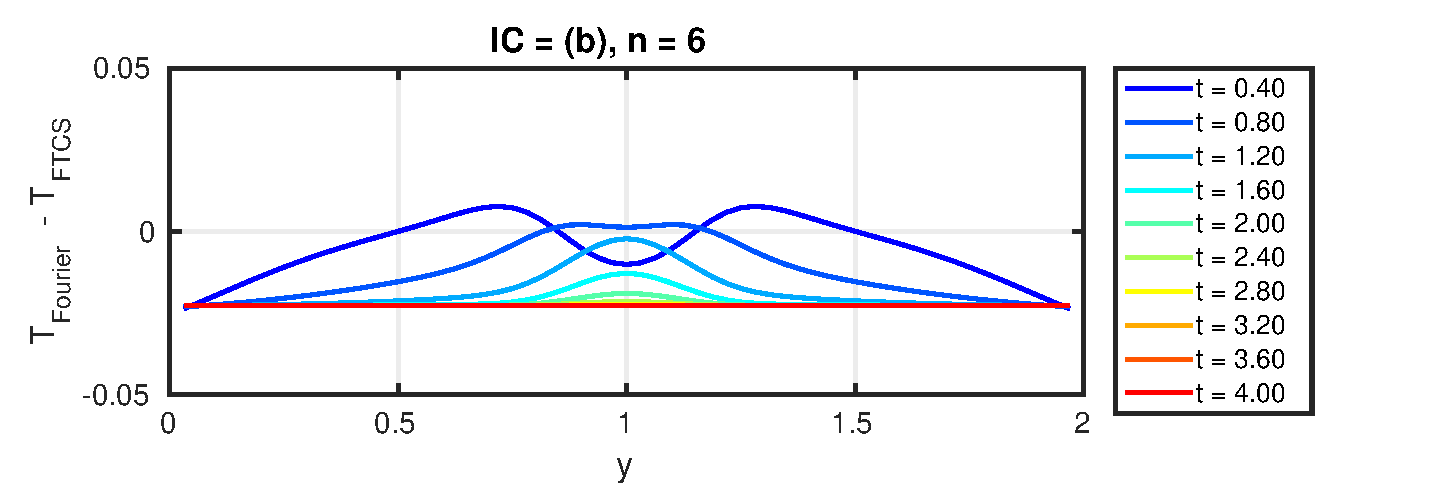
\includegraphics[width=0.85\textwidth]{Prob2_b6_error.eps}
\\[0.5cm]
\caption{Difference between the Fourier pseudo-spectral and FTCS solutions at evenly-spaced discrete times $t<4$, omitting the initial condition. Different initial conditions and spatial resolutions produce different behavior.}
\label{fig:Prob2_error}
\end{center}
\end{figure}

%%%%%%%%%%%%%%%%%%%%%%%%%%%%%%%%%%%%%%%%%%%%%%%%%
%%%%%%%%%%%%%%%%%%%%%%%%%%%%%%%%%%%%%%%%%%%%%%%%%
\section{Discussion} %%%%%%%%%%%%%%%%%%%%%%%%%%%%
%%%%%%%%%%%%%%%%%%%%%%%%%%%%%%%%%%%%%%%%%%%%%%%%%
%%%%%%%%%%%%%%%%%%%%%%%%%%%%%%%%%%%%%%%%%%%%%%%%%

The FTCS method for initial condition (b) has difficulty capturing the diffusive behavior accurately; the limiting Fourier value is $T \sim 0.765$ for both $n=\{5,6\}$, whereas the FTCS method's limiting values are $T \sim \{0.806, 0.788\}$ respectively.

%%%%%%%%%%%%%%%%%%%%%%%%%%%%%%%%%%%%%%%%%%%%%%%%%
%%%%%%%%%%%%%%%%%%%%%%%%%%%%%%%%%%%%%%%%%%%%%%%%%
\section{References} %%%%%%%%%%%%%%%%%%%%%%%%%%%%
%%%%%%%%%%%%%%%%%%%%%%%%%%%%%%%%%%%%%%%%%%%%%%%%%
%%%%%%%%%%%%%%%%%%%%%%%%%%%%%%%%%%%%%%%%%%%%%%%%%

No external references were used other than the course notes for this assignment.

%%%%%%%%%%%%%%%%%%%%%%%%%%%%%%%%%%%%%%%%%%%%%%%%%
%%%%%%%%%%%%%%%%%%%%%%%%%%%%%%%%%%%%%%%%%%%%%%%%%
\section*{Appendix: MATLAB Code} %%%%%%%%%%%%%%%%
%%%%%%%%%%%%%%%%%%%%%%%%%%%%%%%%%%%%%%%%%%%%%%%%%
%%%%%%%%%%%%%%%%%%%%%%%%%%%%%%%%%%%%%%%%%%%%%%%%%

The following code listings generate all figures presented in this homework assignment. The Fourier codes \lstinline|find_dfdn.m| and \lstinline|find_d2fdn2.m| are provided by Prof.\ Biringen.

\includecode{Problem_1.m}
\includecode{find_dfdn.m}
\includecode{find_d2fdn2.m}
\includecode{Problem_2.m}

%%
%% DOCUMENT END
%%
\end{document}
